\documentclass[11pt,fleqn]{article}
%\usepackage{CJK}
\usepackage{latexsym}
\usepackage{color}
\usepackage{graphicx, float}\usepackage{graphicx}
%\usepackage{algorithmicx}
\usepackage{algorithm}
\usepackage{algpseudocode}
%\usepackage[colorlinks]{hyperref}
\setlength{\oddsidemargin}{-0.0in}
\setlength{\evensidemargin}{-0.0in} \setlength{\textwidth}{6.0in}
\setlength{\textheight}{9.0in} \setlength{\topmargin}{-0.2in}

%\setlength{\leftmargin}{0.7in}
\usepackage{amssymb, graphicx, amsmath}  %  fancyheadings,

\newcommand\qed{\qquad $\square$}
\newcommand{\nn}{\nonumber}

\def \[{\begin{equation}}
\def \]{\end{equation}}
\def\proof{{\bf Proof:\quad}}
\def \endzm {\quad $\Box$}
\def\dist{\hbox{dist}}


\newcommand{\R}{\mathbb{R}}
%\newtheorem{yinli}{����}[section]
\newcommand{\D}{\displaystyle}
\newcommand{\T}{\textstyle}
\newcommand{\SC}{\scriptstyle}
\newcommand{\FT}{\footnotesize}



%\newtheorem{theorem}{Theorem}[section]
%\renewcommand{\thetheorem}{\arabic{section}.\arabic{theorem}}
\newtheorem{definition}{Definition}
\renewcommand{\thedefinition}{\arabic{section}.\arabic{definition}}
\newtheorem{lemma}{Lemma}[section]
\renewcommand{\thelemma}{\arabic{section}.\arabic{lemma}}
\newtheorem{remark}{Remark}
\renewcommand{\theremark}{\arabic{section}.\arabic{remark}}
\newtheorem{proposition}{Proposition}[section]
\renewcommand{\theproposition}{\arabic{section}.\arabic{proposition}}
\newtheorem{corollary}{Corollary }[section]
\renewcommand{\thecorollary}{\arabic{section}.\arabic{corollary}}
\renewcommand{\theequation}{\arabic{section}.\arabic{equation}}
\renewcommand{\baselinestretch}{1.35}
\newtheorem{exam}{Example}[section]
\renewcommand{\theexam}{\arabic{section}.\arabic{exam}}
\newtheorem{theo}{Theorem}[section]
\renewcommand{\thetheo}{\arabic{section}.\arabic{theo}}
\begin{document}
%\begin{CJK*}{GBK}{song}

\begin{center}

{\LARGE \bf  Machine Learning and Computer Vision Assignment 3}\\


\vskip 25pt
 {Huihuang Zheng, huihuang@utexas.edu }\\
\vskip 5pt
{\small hz4674 Fall 2015 }


\end{center}
\section{ Programming }
This section explains usage and implementation of my program.\\
Usage: run ./src/\textbf{main.m} \\
If you want to test on your own images: \\
call \textbf{twoImageMosaic}(image1, image2, autoMatch, useRansac).
    \begin{itemize}
      \item image1 and image2 are directory and name of two input images.
      \item autoMatch and useRansac are boolean values to indicate whether use automatically matchin and RANSAC. By default, we use autoMatch but not RANSAC
    \end{itemize}

\subsection{Getting correspondences}
See \textbf{manualCorresp.m}. If you set $autoMatch = false$ in \textbf{twoImageMosaic}. My GUI will show the two images. You need to clikc one point in left image, then corresponding one point in right image. Then the next pair of points. Press Enter when you finish.
\subsection{Computing the homography parameters}
See \textbf{homography.m}. The mathematic behind the program:
$$H =
\begin{pmatrix}
a & b & c \\
d & e & f \\
g & h & 1 \\
\end{pmatrix}
,
p_1 =
\begin{pmatrix}
x\\
y\\
1\\
\end{pmatrix}
,
p_2 =
\begin{pmatrix}
x'\\
y'\\
1\\
\end{pmatrix}
$$
We know $wp_2 = Hp_1$, So
$$x' = (ax + by + c) / w  $$
$$y' = (dx + ey + f) / w  $$
$$w = (gx + hy + 1)$$
From $x' = (ax + by + c) / w$ and $w = (gx + hy + 1) / w$ we have
$$(gx + hy + 1)x' = ax + by + c \Rightarrow x' = ax + by + c - gxx' - hyx'$$
Similarly, from $y' = (dx + ey + f) / w  $ and $w = (gx + hy + 1) / w$ we have
$$(gx + hy + 1)y' = dx + ey + f \Rightarrow y' = dx + ey + f - gxy' - hyy$$
We know points $x, y, x', y'$. We just need to find parameters of $H$:
$$
\begin{pmatrix}
x & y & 1 & 0 & 0 & 0 & -xx' & -yx' \\
0 & 0 & 0 & x & y & 1 & -xy' & -yy' \\
...
\end{pmatrix}
\begin{pmatrix}
a \\ b \\ c \\ d \\ e \\ f \\ g \\ h
\end{pmatrix}
=
\begin{pmatrix}
x'\\
y'\\
...
\end{pmatrix}
$$
\subsection{Warping between image planes}
See \textbf{warpImage.m}, for every pixel in warped image, I inverse the coordinate to the input image. Then the pixel's value is the interpolate value in input image.  In here we need to compute inverse of homography transformation. Say it in mathematic way: $wp_2 = Hp_1$. We know $H$ and $p_2$ and we want to compute $p_1$: $H^{-1}wp_2 = p_1 $, so $ H^{-1}p_2 = \frac{1}{w}p_1$. How can we know $w$? The third entry of $p_1$ is one! We just compute $H^{-1}p_2$, then the third entry of $H^{-1}p_2$ is $\frac{1}{w}$, Then we can get $p_1$.
\subsection{Create the output mosaic}
See \textbf{mosaic.m}, this function is easy, just put one warped image and anther image together.
\section{ Answer Question}
\subsection{Output Mosaic}
See my result mosaic of two provided UT tower images in figure \ref{mosaic}.
\begin{figure}
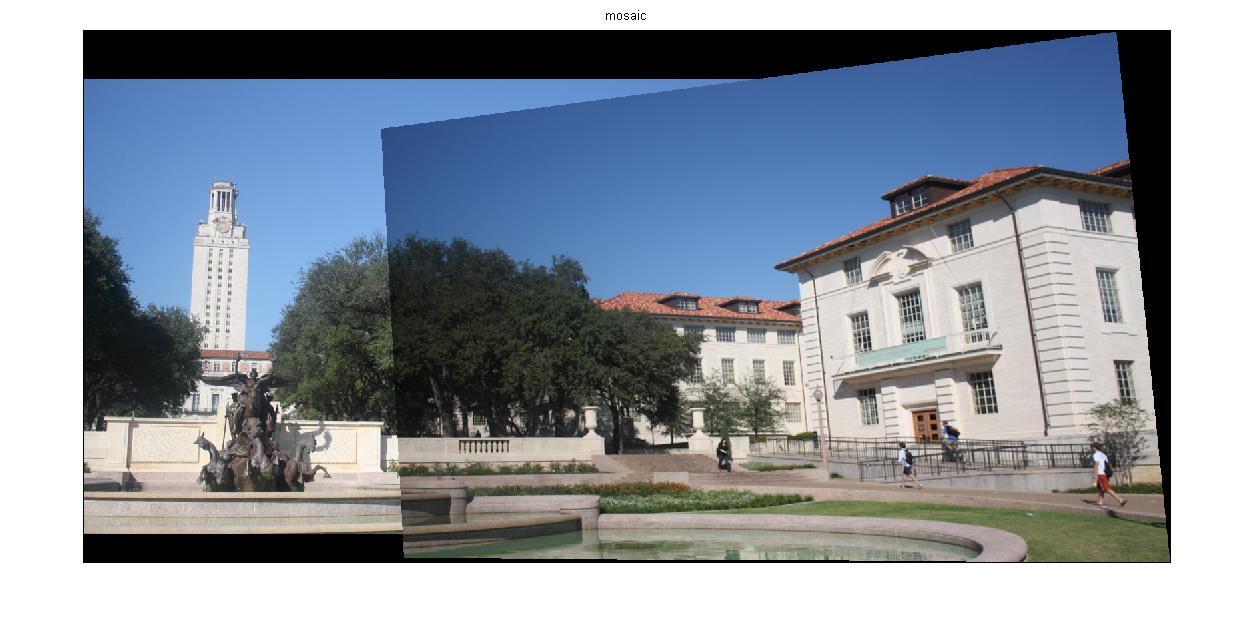
\includegraphics[width = 1.2\linewidth]{mosaic1.jpg}
\caption{Mosaic of Two Provided Images}
\label{mosaic}
\end{figure}
\subsection{Additional Example}
See images of my room in figure \ref{myroom}, and mosaic result in figure \ref{myroomMosaic}
\begin{figure}
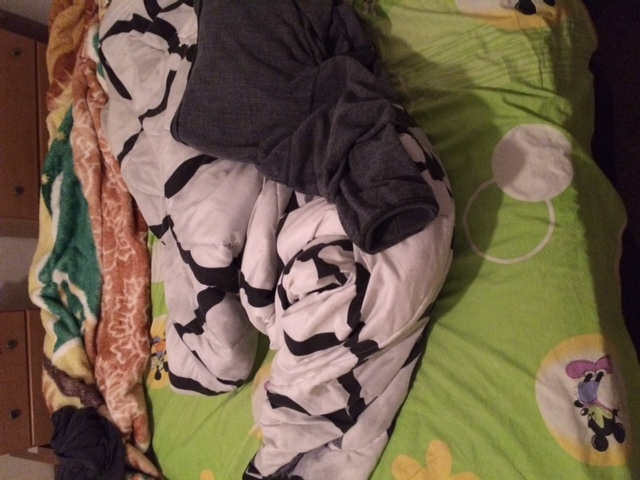
\includegraphics[width = 0.8\linewidth]{myroom1.jpg}
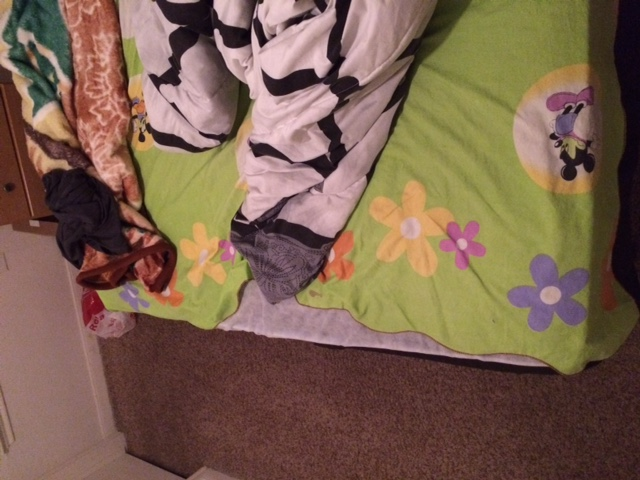
\includegraphics[width = 0.8\linewidth]{myroom2.jpg}

\caption{My Room Images}
\label{myroom}
\end{figure}

\begin{figure}

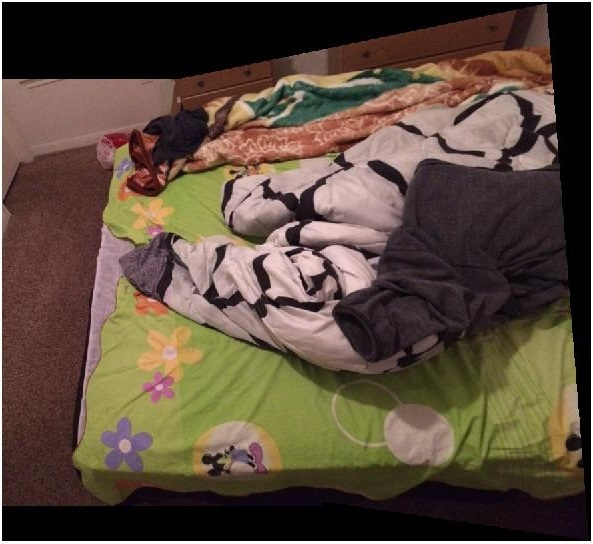
\includegraphics[width = 0.8\linewidth]{myroom3.jpg}
\caption{My Room Images Mosaic}
\label{myroomMosaic}
\end{figure}

\subsection{Behavior of Automatically Matching}
I found that the most important thing of SIFT automatically matching in this program assignment is the uniqueness of matching. In my experiment, when I started to use \emph{vl\_sift} and \emph{vl\_ubcmatch} at first, because I set small threshold in \emph{vl\_ubcmatch} (here, threshold means: A descriptor D1 is matched to a descriptor D2 only if the distance d(D1,D2) multiplied by threshold is not greater than the distance of D1 to all other descriptors). The small value (like the default value of 1.5) will cause result like figure \ref{doeantwork}. Then I used high value like 5, 10 and got right result in question 2.1 figure \ref{mosaic}
\begin{figure}
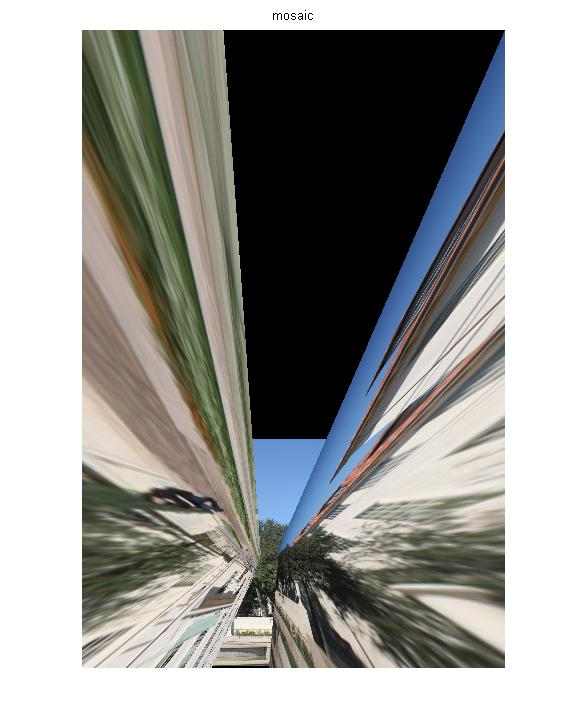
\includegraphics[width = 0.8\linewidth]{doesntWork.jpg}
\caption{Small Threshold Doesn't Work}
\label{doeantwork}
\end{figure}

\subsection{Warp into a frame}
I used two images: my photo and a photo of Kristen's class in figure \ref{kristenMeInput}. The result is in figure \ref{kristenMe}. To obtain this is easy. Using manual click, let the points from the one view be the corners of the image you want to insert in the frame, and the let the corresponding points in the second view be the clicked points of the frame. I clicked on four vertexes of my photo and four corner points in Kristen's slide, the output image is just like that.
\begin{figure}
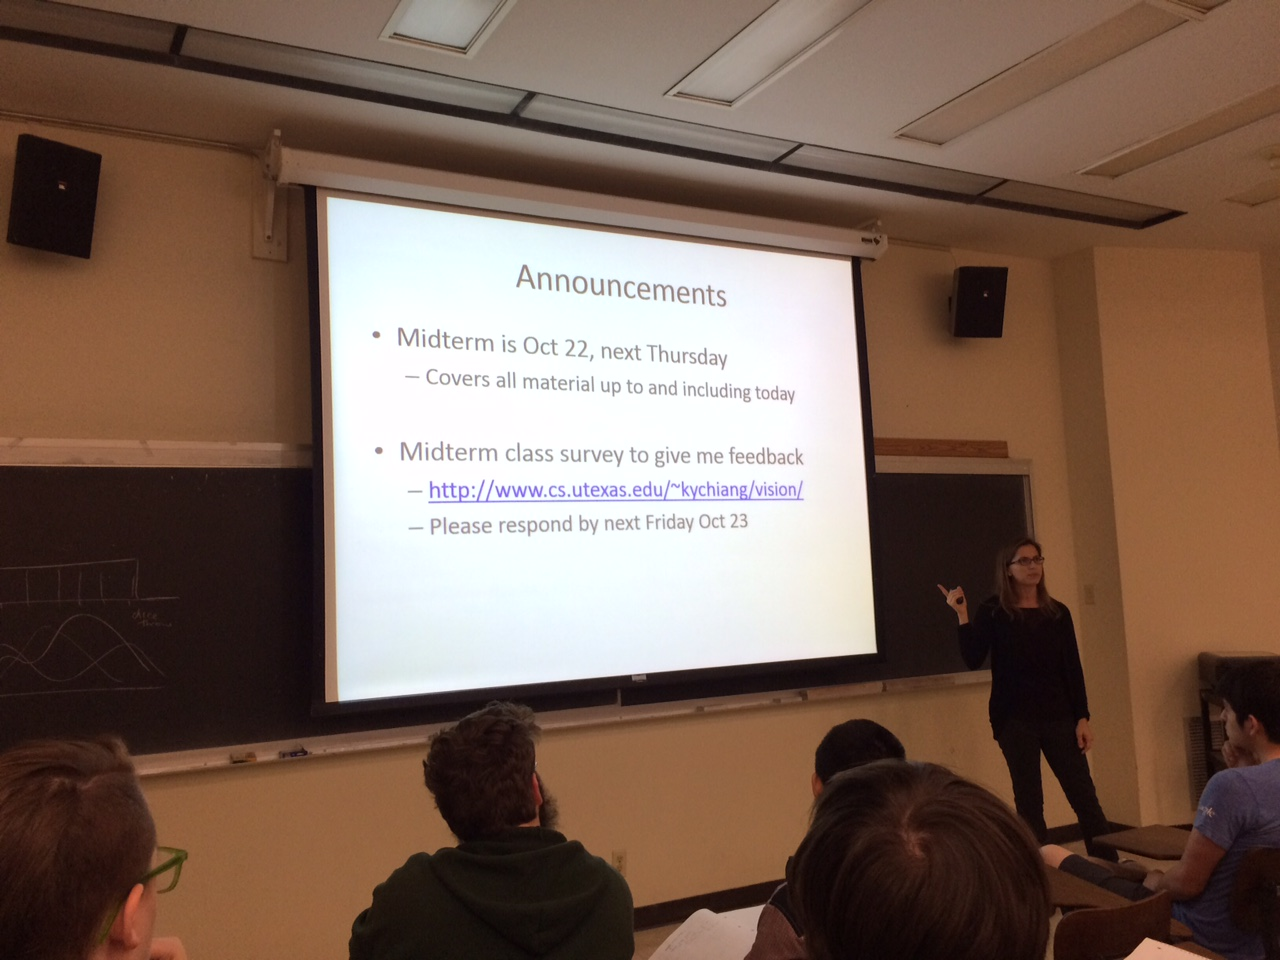
\includegraphics[width = 0.8\linewidth]{KristenClass.jpg}
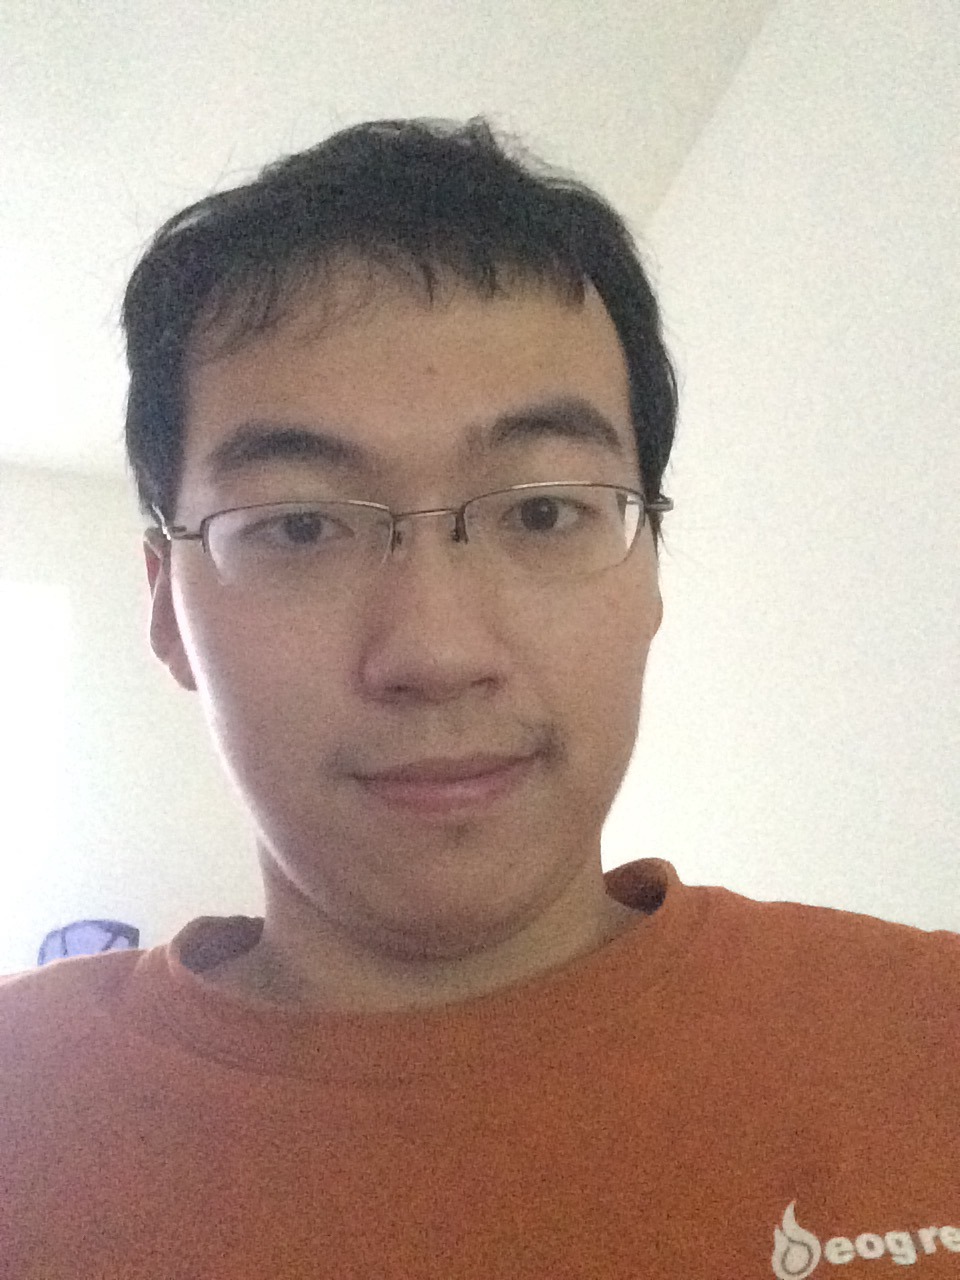
\includegraphics[width = 0.6\linewidth]{meHuihuangZheng.jpg}
\caption{Two input images}
\label{kristenMeInput}
\end{figure}

\begin{figure}
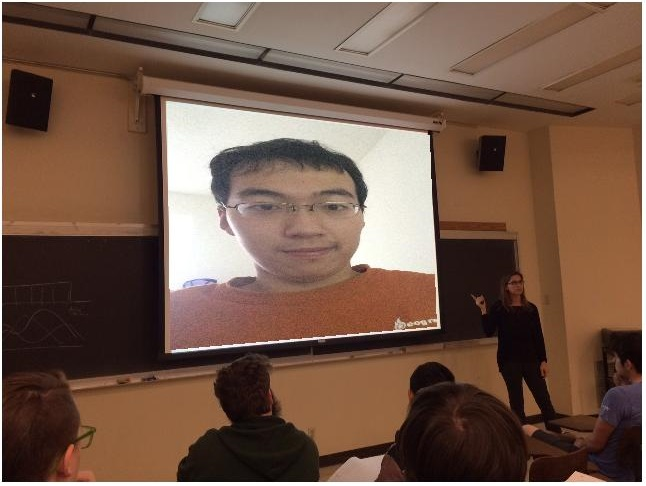
\includegraphics[width = 1.1\linewidth]{KristenAndMe.jpg}
\caption{I'm in class image}
\label{kristenMe}
\end{figure}
\section{ Extra Credit }

\subsection{RANSAC}
See \textbf{ransac.m}. In fact, there are many bad matched features of SIFT between uttower1.jpg and uttower2.jpg. For example, I rand chose four matched features to get homography, it may come out bad example (figure \ref{badexample}). Using RANSAC, I got different result compared to using all matched features (figure \ref{ransac}). 
\begin{figure}
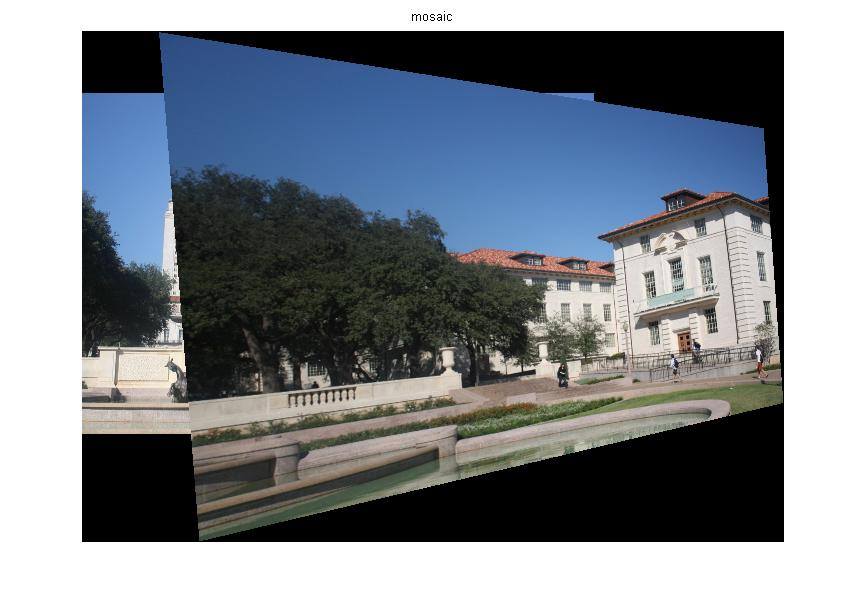
\includegraphics[width = 1.1\linewidth]{badexample.jpg}
\caption{A Bad Example of Feature Matching betweern uttower1,2.jpg}
\label{badexample}
\end{figure}

\begin{figure}
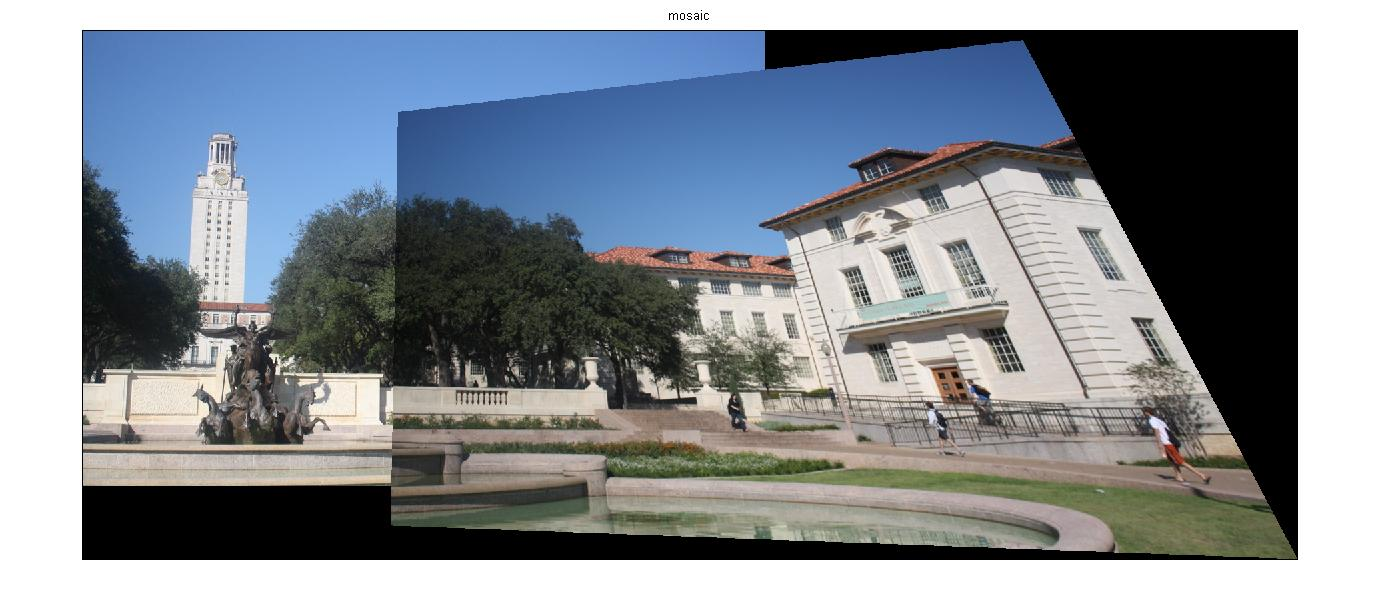
\includegraphics[width = 1.1\linewidth]{ransac.jpg}
\caption{RANSAC result}
\label{ransac}
\end{figure}

\subsection{Rectify}
See \textbf{rectify.m}. Using my rectify function, you need to choose 4 points in the imags by clicking four corner points, order: top left, bottom left, top right, bottom right. Then press Enter. The output image is square picture. \\
I used uttower1.jpg (figure \ref{uttower1}) as example, the door on second floor of right house is oblique. I choose four points surrounding the second floor, and outputs square result of it (figure \ref{rectify}).
\begin{figure}
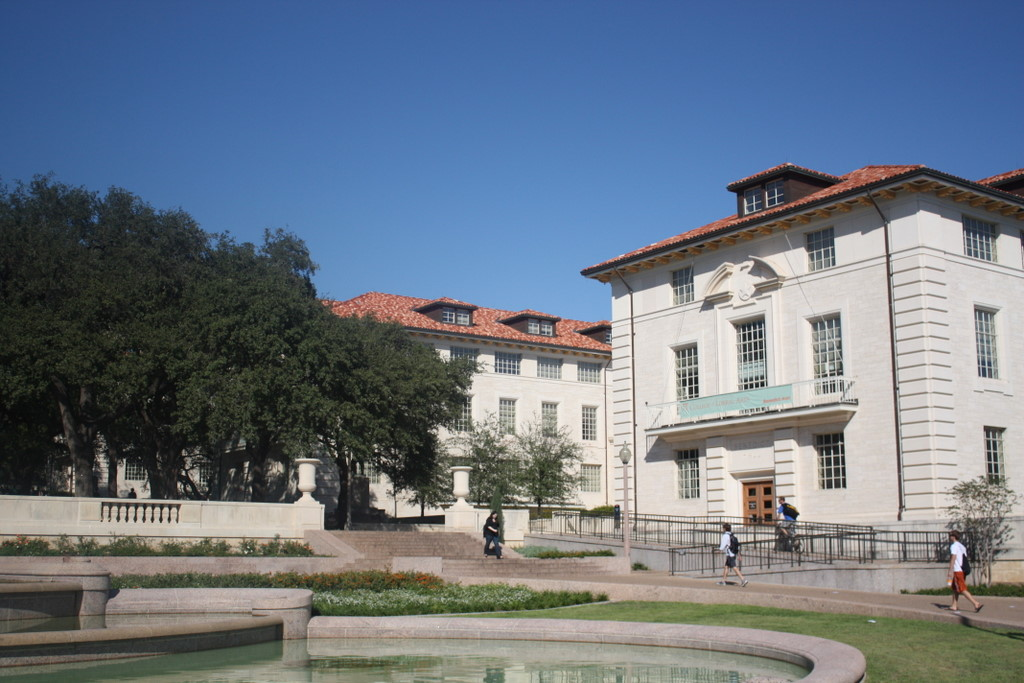
\includegraphics[width = 1.1\linewidth]{uttower1.jpg}
\caption{uttower1.jpg}
\label{uttower1}
\end{figure}

\begin{figure}
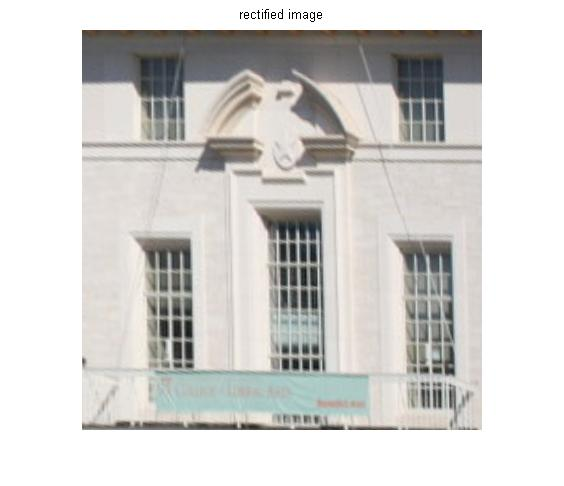
\includegraphics[width = 1.1\linewidth]{rectified.jpg}
\caption{Rectified Image of door in right of uttower1.jpg}
\label{rectify}
\end{figure}
%\end{CJK*}
\end{document}
